\def\CLASSINPUTinnersidemargin{19mm}
\def\CLASSINPUToutersidemargin{19mm}
\def\CLASSINPUTtoptextmargin{25mm}
\def\CLASSINPUTbottomtextmargin{31mm}
\documentclass[a4paper,conference]{IEEEtran}
\IEEEoverridecommandlockouts

\usepackage{cite}
\usepackage{amsmath,amssymb,amsfonts}
\usepackage{graphicx}
\usepackage{textcomp}
\usepackage{xcolor}
\usepackage{booktabs}
\usepackage{array}
\usepackage{url}
\usepackage{hyperref}
\hypersetup{hidelinks}
\setlength{\columnsep}{6mm}
\AtBeginDocument{%
  \typeout{IEEM layout check: paper=\the\paperwidth\space x \the\paperheight; text=\the\textwidth\space x \the\textheight; columnsep=\the\columnsep; columnwidth=\the\columnwidth.}%
}

\graphicspath{{../figures/}}

\begin{document}

\title{\fontsize{14}{17}\selectfont\bfseries CONFOUNDER-AWARE ECO-DRIVING DECISION SUPPORT\\ FOR SIMULATED URBAN LOGISTICS}

\author{
\IEEEauthorblockN{M. R. Alamudi\IEEEauthorrefmark{1},
H. Wicaksono\IEEEauthorrefmark{2},
K. A. Prayitno\IEEEauthorrefmark{3}}
\IEEEauthorblockA{\IEEEauthorrefmark{1}Department of Computer Sciences and Electronics, Gadjah Mada University, Yogyakarta, Indonesia\\
\IEEEauthorrefmark{2}School of Business, Social, and Decision Sciences, Constructor University, Bremen, Germany\\
\IEEEauthorrefmark{3}Politeknik ATK Yogyakarta, Yogyakarta, Indonesia\\
(razan@madrazaldi.dev, h.wicaksono@constructor.university, kututaji@politeknikatk.ac.id)}
}

\maketitle

\begin{abstract}
Urban logistics operators need low-emission driving decisions that do not compromise service or safety, but online experimentation is costly and historical choices are confounded by urgency, congestion, weather, and route conditions. We study eco-mode selection as offline policy learning on a synthetic urban logistics log of 96{,}000 decision epochs across 120 days, 120 vehicles, and 15 zones. The pipeline combines a deployable confounder-aware state, fitted Q iteration (FQI), validation-selected support-constrained overrides, and per-decision doubly robust off-policy evaluation. After excluding outcome-adjacent proxy fields, confounder-aware FQI improves by point estimate over the proxy-rich FQI comparator ($-4.694$ vs.\ $-4.712$), held-out logged-action replay ($-4.826$), and a 5-feature minimal baseline ($-4.810$). A validation-frozen heuristic risk rule remains strongest ($-4.636$, 95\% CI $[-4.782, -4.495]$), so this is not a universal dominance claim. The contribution is an audit-backed synthetic benchmark and support-constrained decision-support workflow, with explicit boundaries separating deployable recommendations from deployment-ready autonomous control.
\end{abstract}

\renewcommand\IEEEkeywordsname{Keywords}
\begin{IEEEkeywords}
Causal inference, off-policy evaluation, offline policy learning, urban logistics
\end{IEEEkeywords}

\section{Introduction}
Urban last-mile logistics must reduce emissions and fuel use without degrading service reliability or safety \cite{demir_green_2014,dekker2012or}. Existing logistics analytics largely focuses on ETA prediction, travel-time forecasting, routing, or emissions estimation \cite{derrow2021eta,wang2019simple,li2018dcrnn,toth2014vrp}. Those tools support planning, but they do not learn \emph{operational actions} directly from logged behavior.

Historical operational logs can support reinforcement-learning decisions, but their action-outcome patterns are not automatically causal \cite{pearl2009causality,hernan2020causal,lu2018deconfounding}. Traffic, weather, route characteristics, delivery urgency, vehicle condition, and prior service history may affect both eco-driving decisions and service, safety, and emissions outcomes. A confounder-aware representation records deployable pre-decision context, excludes outcome-adjacent proxies, and makes the policy-learning audit explicit.

We study whether to activate eco mode on a trip segment. Because live experimentation is costly, this is an offline decision-learning problem with observational bias. Batch policy-learning tools such as FQI provide a useful template \cite{levine2020offline,ernst2005tree,fujimoto2019bcq}, but they are vulnerable to extrapolation and low-support errors \cite{kumar2020cql,laroche2019spibb,prudencio2023survey}. Our approach combines conservative policy improvement with a deployable state motivated by causal adjustment ideas \cite{pearl2009causality,hernan2020causal,bareinboim2016causal,zhang2019dtr,lu2018deconfounding}.

\paragraph*{Research question} In a synthetic urban logistics case study, can confounder-aware offline policy learning provide credible decision support for eco-mode selection relative to held-out logged-action replay, heuristic rules, and a broader non-causal comparator?

\paragraph*{Contributions} We cast eco-mode selection as offline policy learning over vehicle-day logs, build an auditable benchmark with confounder-aware and non-causal comparators, and show that confounder-aware FQI improves by point estimate over logged-action replay and the proxy-audited non-causal FQI comparator. Heuristic and ablated policies can remain stronger, making the contribution a claim-bounded decision-support workflow rather than a full-policy dominance result.

\section{Related Work and Research Gap}
\label{sec:related}
The closest logistics literature emphasizes prediction and planning rather than policy learning. ETA and travel-time forecasting use boosted and deep models \cite{derrow2021eta,wang2019simple,li2018dcrnn}; routing and service planning emphasize combinatorial optimization \cite{toth2014vrp}; green logistics studies focus on fuel and emissions trade-offs \cite{dekker2012or,demir_green_2014,eglese2014green}. Taken together, this adjacent literature leaves a gap for learning action policies directly from logged operational decisions.

Offline policy learning from fixed logs draws on batch reinforcement learning and conservative policy-improvement methods \cite{levine2020offline,ernst2005tree,fujimoto2019bcq}, but strong performance depends on overlap and conservative improvement \cite{kumar2020cql,laroche2019spibb,thomas2015hcpi,prudencio2023survey}; in observational settings, state design also has to account for confounding structure \cite{pearl2009causality,hernan2020causal,lu2018deconfounding}. The area has prominent healthcare applications and safety-oriented methodological guidance \cite{komorowski2018sepsis,gottesman2019guidelines} but remains sparse in urban logistics. Off-policy evaluation is therefore essential, with early foundations in off-policy value estimation \cite{precup2000op}; we use doubly robust estimation as the headline per-decision metric, with inverse-propensity and FQE diagnostics \cite{dudik2011dr,jiang2016doubly,thomas2016dataefficient,le2019batch,kallus2020double}.

Causal inference is used as state-design discipline: it motivates a deployable pre-decision state and excludes post-action outcomes and non-deployable latent variables \cite{pearl2009causality,hernan2020causal,bareinboim2016causal,lu2018deconfounding}. Recent open work frames causal artificial intelligence as a candidate tool for collaborative urban-logistics sustainability analysis \cite{prayitno2024framework}, and a logistics-focused review identifies causal RL as a promising route toward more explainable collaborative urban-logistics decisions \cite{prayitno2024causalrlreview}. The goal is an auditable decision-support design, not general causal optimality.

\section{Problem Formulation and Proposed Method}
\label{sec:method}

\subsection{Historical Data and Log Generation}
We formulate eco-mode control as offline policy learning over vehicle-day logs. Each row is one synthetic dispatch decision for one vehicle in one zone; trajectories use (\texttt{date}, \texttt{vehicle\_id}); and \texttt{eco\_mode} is a binary action. The source artifact exposes the schema, data dictionary, and outcomes, but not the simulator equations, so the main study is a log-level benchmark rather than a claim about known structural eco-mode effects.

\subsection{Confounder-Aware State Representation}
The state is deployable pre-decision context that may affect both action choice and outcomes: time, vehicle, demand, service-window, road, weather, traffic, route-risk, dispatch-delay, trajectory-position, and rolling history fields. Outcome variables, post-action measurements, and simulator-only latent variables are excluded. This does not prove that all backdoor paths are blocked; it makes the adjustment assumptions auditable and prevents recommendation-time leakage.

\begin{table}[t]
\caption{Synthetic Benchmark and State Use}
\label{tab:benchmark_design}
\centering
\scriptsize
\renewcommand{\arraystretch}{0.98}
\setlength{\tabcolsep}{3pt}
\begin{tabular}{>{\raggedright\arraybackslash}p{0.27\columnwidth}>{\raggedright\arraybackslash}p{0.67\columnwidth}}
\toprule
\textbf{Component} & \textbf{Specification} \\
\midrule
Observed confounding & Historical choices are observational and may depend on time, vehicle, demand, traffic, weather, route, and prior context; latent maintenance, driver-skill, and driver-risk fields are not deployable. \\
Causal roles & Treatment/action $A$ is \texttt{eco\_mode}; headline outcome $Y$ is \texttt{reward\_primary}; component outcomes are \texttt{lateness\_min}, \texttt{crash}, \texttt{near\_miss}, and \texttt{co2\_kg}; observed adjustment set $Z$ is the pre-decision deployable context. \\
Confounder-aware state & \texttt{day\_idx}, \texttt{dow}, \texttt{hour}, \texttt{zone}, vehicle type/age/efficiency, commodity/demand/window/service fields, road/weather/traffic fields, \texttt{route\_risky}, \texttt{dispatch\_delay\_min}, \texttt{step\_idx}, \texttt{remaining\_steps}, and rolling/prior traffic, lateness, incident, reward, and action features. \\
Policy/nuisance use & Confounder-aware FQI, its logging/FQE/DR nuisance models, and the heuristic rule use the deployable state; DR outcome inputs add only candidate \texttt{eco\_mode}. Non-causal FQI and its logging/FQE/DR nuisance models add \texttt{compatibility\_violation}. \\
Ablations & No-history removes rolling/prior features; no-vehicle removes \texttt{vehicle\_id}; minimal FQI uses \texttt{hour}, \texttt{demand\_size}, \texttt{time\_window\_tightness}, \texttt{traffic\_index}, and \texttt{dispatch\_delay\_min}; latent oracle is diagnostic only. \\
Excluded fields & Post-action/proxy fields \texttt{avg\_speed\_kmph}, \texttt{travel\_time\_min}, \texttt{fuel\_liters}, \texttt{co2\_kg}, \texttt{crash}, \texttt{near\_miss}, \texttt{lateness\_min}, \texttt{on\_time}, \texttt{distance\_km}, \texttt{risk\_score}, and latent simulator columns. \\
\bottomrule
\end{tabular}
\end{table}

\subsection{Reward Specification}
The primary reward balances service, safety, and sustainability:
\begin{equation}
r_t = -\big( \ell_t + \alpha c_t + \beta n_t + \gamma e_t \big),
\label{eq:primary_reward}
\end{equation}
where $\ell_t$ is lateness, $c_t$ and $n_t$ are crash and near-miss indicators, $e_t$ is emitted CO\textsubscript{2}, and $(\alpha,\beta,\gamma)=(10,2,0.2)$. The reward-weight symbol $\gamma$ is distinct from the FQI discount factor used below. Service-heavy and sustainability-heavy rewards are used as sensitivity checks.
The constants are a priori lateness-minute-equivalent utility tradeoffs, not estimated from deployment costs: one crash is 10 lateness minutes, one near miss is 2, and 1 kg CO\textsubscript{2} is 0.2. As configured coefficient shares, these weights sum to 100\% as 7.6\% lateness, 75.8\% crash, 15.2\% near miss, and 1.5\% CO\textsubscript{2}. The repository file \texttt{reward\_weight\_calibration.csv} reports both these normalized coefficient shares and the mean weighted-penalty shares observed on the calibration split.

\subsection{Policy Learning}
Historical eco-mode decisions are observational: urgency, congestion, weather, and route conditions affect both action choice and outcomes. We therefore use the domain-guided pre-decision adjustment set in Table~\ref{tab:benchmark_design}; because three simulator-only latent variables remain unavailable, the backdoor condition is an explicit claim boundary rather than a formal identification result.

We estimate the logging policy with calibrated logistic regression and train deterministic policies with FQI \cite{ernst2005tree}. FQI and FQE use next-state fields and vehicle-day context, but the headline comparison is per-decision decision support under fixed logged contexts.

\subsection{Recommendation Generation}
The recommendation layer is a policy-improvement overlay, not a standalone autonomous policy. It takes a deployable state and baseline proposal $a_t^{\text{base}}$; in held-out evaluation this baseline is the logged action. To avoid weakly supported actions \cite{laroche2019spibb,thomas2015hcpi}, let $a_t^\star = \arg\max_a \hat{Q}(s_t, a)$ and $\Delta_t = |\hat{Q}(s_t, 1) - \hat{Q}(s_t, 0)|$. The overlay recommends
\begin{equation}
\pi_{\text{safe}}(s_t, a_t^{\text{base}}) =
\begin{cases}
a_t^\star, & \hat{\mu}(a_t^\star \mid s_t) \!\ge\! \tau_\mu \text{ and } \Delta_t \!\ge\! \tau_Q, \\
a_t^{\text{base}}, & \text{otherwise},
\end{cases}
\label{eq:safe}
\end{equation}
with validation-selected thresholds $(\tau_\mu, \tau_Q) = (0.05, 0.50)$ fixed on the test set. Baselines are logged replay, always-eco, never-eco, and a validation-frozen heuristic risk rule. The heuristic is not RL: it estimates $\hat{p}_{late}(s)$ on the confounder-aware state, freezes the validation 60th-percentile risk cutoff (0.117), and uses $\pi_h(s)=\mathbb{I}\{\hat{p}_{late}(s)<0.117\}$. Logged-action replay reuses observed held-out actions and is not a learned deployable policy.

Figure~\ref{fig:workflow} summarizes the workflow; each stage writes auditable repository artifacts.

\begin{figure}[t]
\centerline{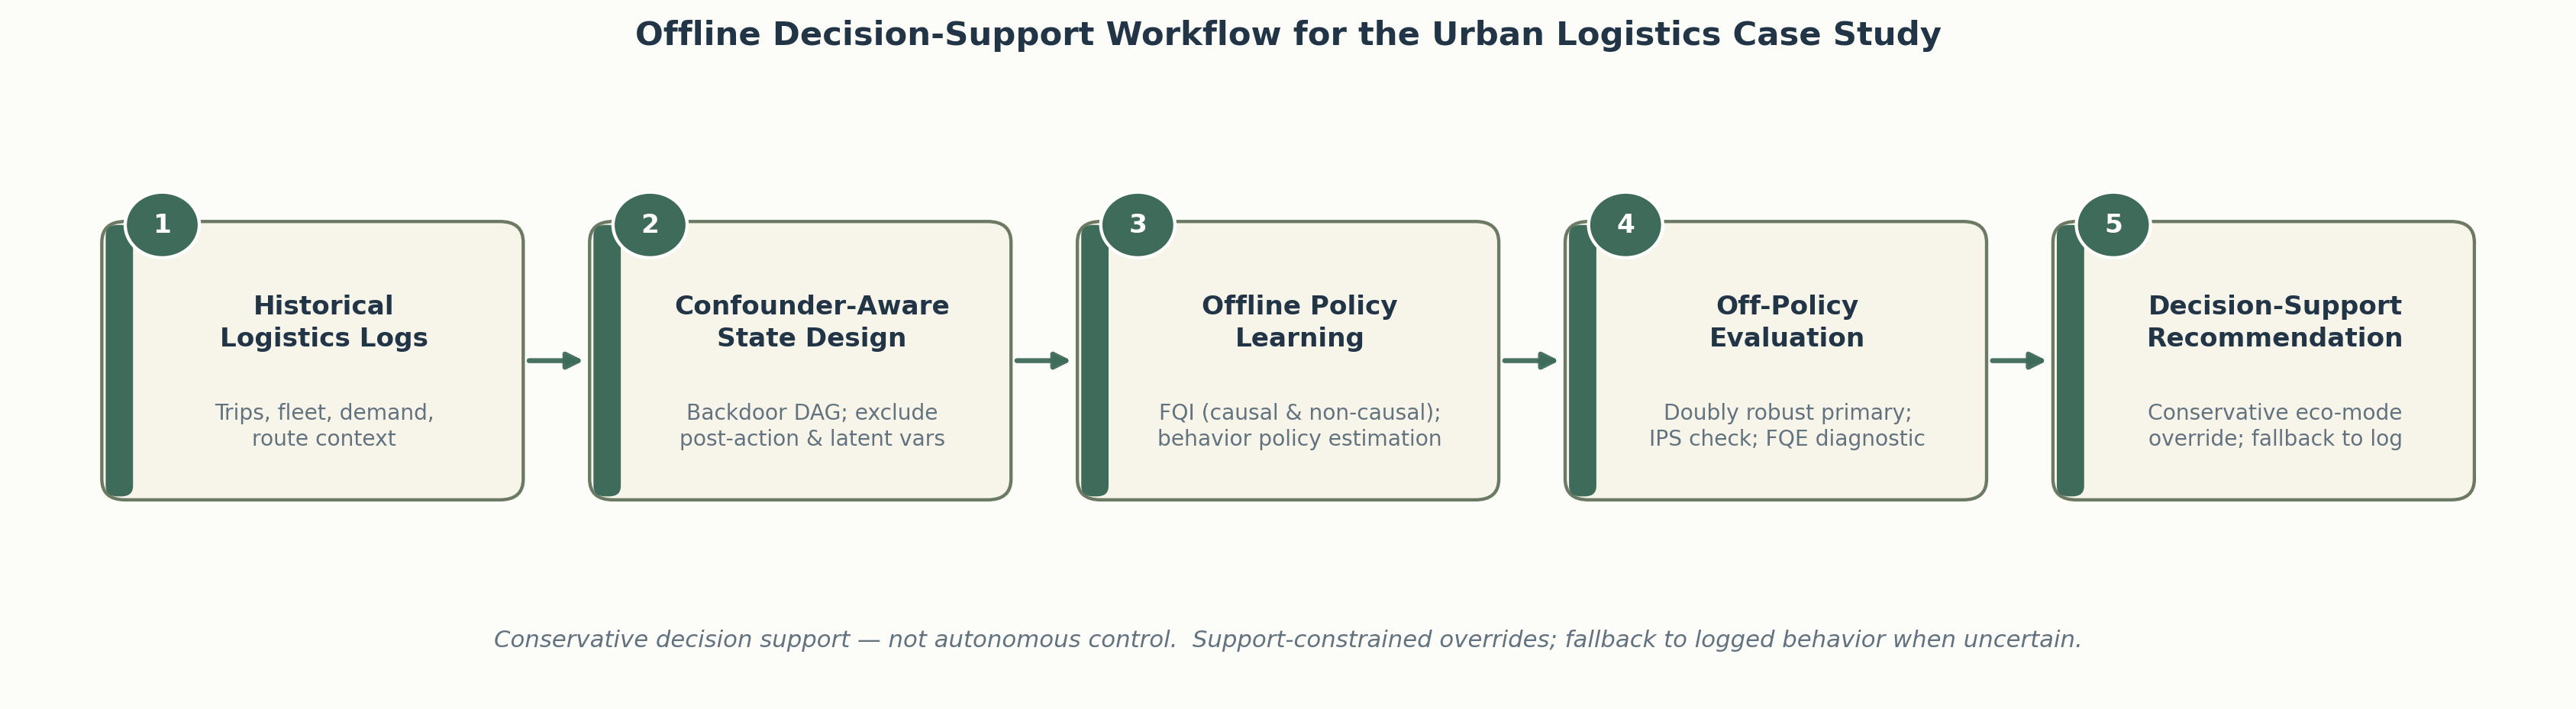
\includegraphics[width=0.9\columnwidth]{workflow.png}}
\caption{Offline decision-support workflow. The recommendation stage changes a baseline action only when value-gap and support gates clear validation-selected thresholds.}
\label{fig:workflow}
\end{figure}

\section{Experimental Setup}
\label{sec:experiments}

The case study uses a synthetic dataset with 96{,}000 rows across 120 dates, 120 vehicles, and 15 zones. Trajectories are sorted by \texttt{date}, \texttt{vehicle\_id}, \texttt{hour}, and source-row order; 19.4\% of date-vehicle-hour groups contain multiple rows, so within-hour ordering is an explicit tie-break assumption. The temporal split is 67{,}179 training rows, 14{,}561 validation rows, and 14{,}260 test rows. The implementation uses Python 3.12, \texttt{pandas}, \texttt{numpy}, \texttt{scikit-learn}, \texttt{matplotlib}, \texttt{seaborn}, and \texttt{joblib}, with fixed seed 42.

Implementation details are fixed before test evaluation: FQI uses $\gamma=0.95$, five Bellman iterations, and action-specific histogram gradient-boosting regressors (depth 6, learning rate 0.05, 120 iterations). FQE uses the same regressor class for 10 iterations; DR outcome models use histogram gradient boosting; and the logging policy is calibrated logistic regression.

Public repository: \url{https://github.com/madrazaldi/Causal-RL}. The Makefile release target rebuilds the log, models, tables, figures, and manuscript; checks cover the manuscript build and page-limit constraints, while the pipeline code records the split, trajectory, leakage-exclusion, threshold, and bootstrap settings used to generate the artifacts.

\subsection{Off-Policy Evaluation Audit}
Policy comparison uses OPE. The headline estimand is not the full closed-loop return over newly generated trajectories; it is the per-decision value of replacing logged decisions under fixed historical contexts, with DR correction for logged-action selection. Let $a_i^\pi=\pi(s_i)$ for standalone baselines and $a_i^\pi=\pi_{\text{safe}}(s_i,a_i^{\text{log}})$ for the overlay. Let $\tilde{\mu}_i=\max\{\hat{\mu}(a_i \mid s_i),10^{-6}\}$ denote the clipped logged-action propensity used in the implementation:
\begin{align}
\hat{V}_{\text{DR}}(\pi) = \frac{1}{n}\sum_i \Bigg[ &\hat{r}(s_i, a_i^\pi) \nonumber \\
&+ \frac{\mathbb{I}\{a_i^\pi = a_i\}}{\tilde{\mu}_i} \big(r_i - \hat{r}(s_i, a_i)\big) \Bigg].
\label{eq:dr}
\end{align}
The same clipped denominator is used for self-normalized IPS. We also compute plug-in and FQE diagnostics \cite{dudik2011dr,jiang2016doubly,thomas2016dataefficient,le2019batch,kallus2020double}. FQE is a discounted trajectory-return diagnostic; DR is the per-decision headline metric. Uncertainty uses 500 bootstrap replicates, including trajectory-level cluster intervals that are 4.3\% wider on average than row-level intervals for the overall primary DR metric, plus paired cluster intervals for key gaps. Robustness slices are high traffic, rain/event, tight window, and late day.

\section{Results and Discussion}
\label{sec:results}

\subsection{Main Policy Comparison}
Table~\ref{tab:main} and Fig.~\ref{fig:policy_values} summarize held-out per-decision DR values. The heuristic rule remains strongest by point estimate ($-4.636$, 95\% CI $[-4.782, -4.495]$). Confounder-aware FQI improves over logged replay ($-4.694$ vs.\ $-4.826$) and the proxy-rich non-causal FQI comparator ($-4.712$) after excluding \texttt{distance\_km} and \texttt{risk\_score}. \texttt{never\_eco} is close at $-4.692$, and paired cluster intervals for the confounder-aware gaps include zero: $[-0.070,0.115]$ versus non-causal FQI and $[-0.001,0.279]$ versus logged replay. The differences are descriptive rather than statistically decisive.

Table and figure labels use the same naming convention. Logged replay reuses observed actions; the heuristic uses a validation-frozen lateness-risk cutoff; confounder-aware FQI uses the full deployable state; no-vehicle and no-history ablations remove vehicle identity and rolling/prior-history fields; minimal FQI uses five operational fields; and non-causal FQI keeps the compatibility flag. The heuristic turns eco mode on for all five lowest lateness-risk deciles, most of the sixth, and none of the top four deciles; its action agreement with full confounder-aware FQI is 0.601.

\begin{table}[t]
\caption{Per-Decision Policy Comparison on the Held-Out Test Set (Primary Reward, Higher Is Better)}
\label{tab:main}
\centering
\scriptsize
\renewcommand{\arraystretch}{1.08}
\setlength{\tabcolsep}{2pt}
\begin{tabular}{lccc}
\toprule
\textbf{Policy} & $\hat{V}_{\text{DR}}$ & \textbf{95\% CI} & \textbf{eco rate} \\
\midrule
Heuristic rule       & $-4.636$ & $[-4.782,\, -4.495]$ & 0.596 \\
Conf.-aware FQI no vehicle & $-4.670$ & $[-4.847,\, -4.486]$ & 0.483 \\
Conf.-aware FQI no history & $-4.687$ & $[-4.862,\, -4.502]$ & 0.486 \\
Never eco            & $-4.692$ & $[-4.891,\, -4.517]$ & 0.000 \\
Conf.-aware FQI      & $-4.694$ & $[-4.886,\, -4.530]$ & 0.478 \\
Non-causal FQI       & $-4.712$ & $[-4.895,\, -4.543]$ & 0.499 \\
Minimal FQI          & $-4.810$ & $[-4.988,\, -4.601]$ & 0.483 \\
Logged replay        & $-4.826$ & $[-5.055,\, -4.577]$ & 0.574 \\
Always eco           & $-5.061$ & $[-5.221,\, -4.914]$ & 1.000 \\
\bottomrule
\end{tabular}
\end{table}

\begin{figure}[t]
\centerline{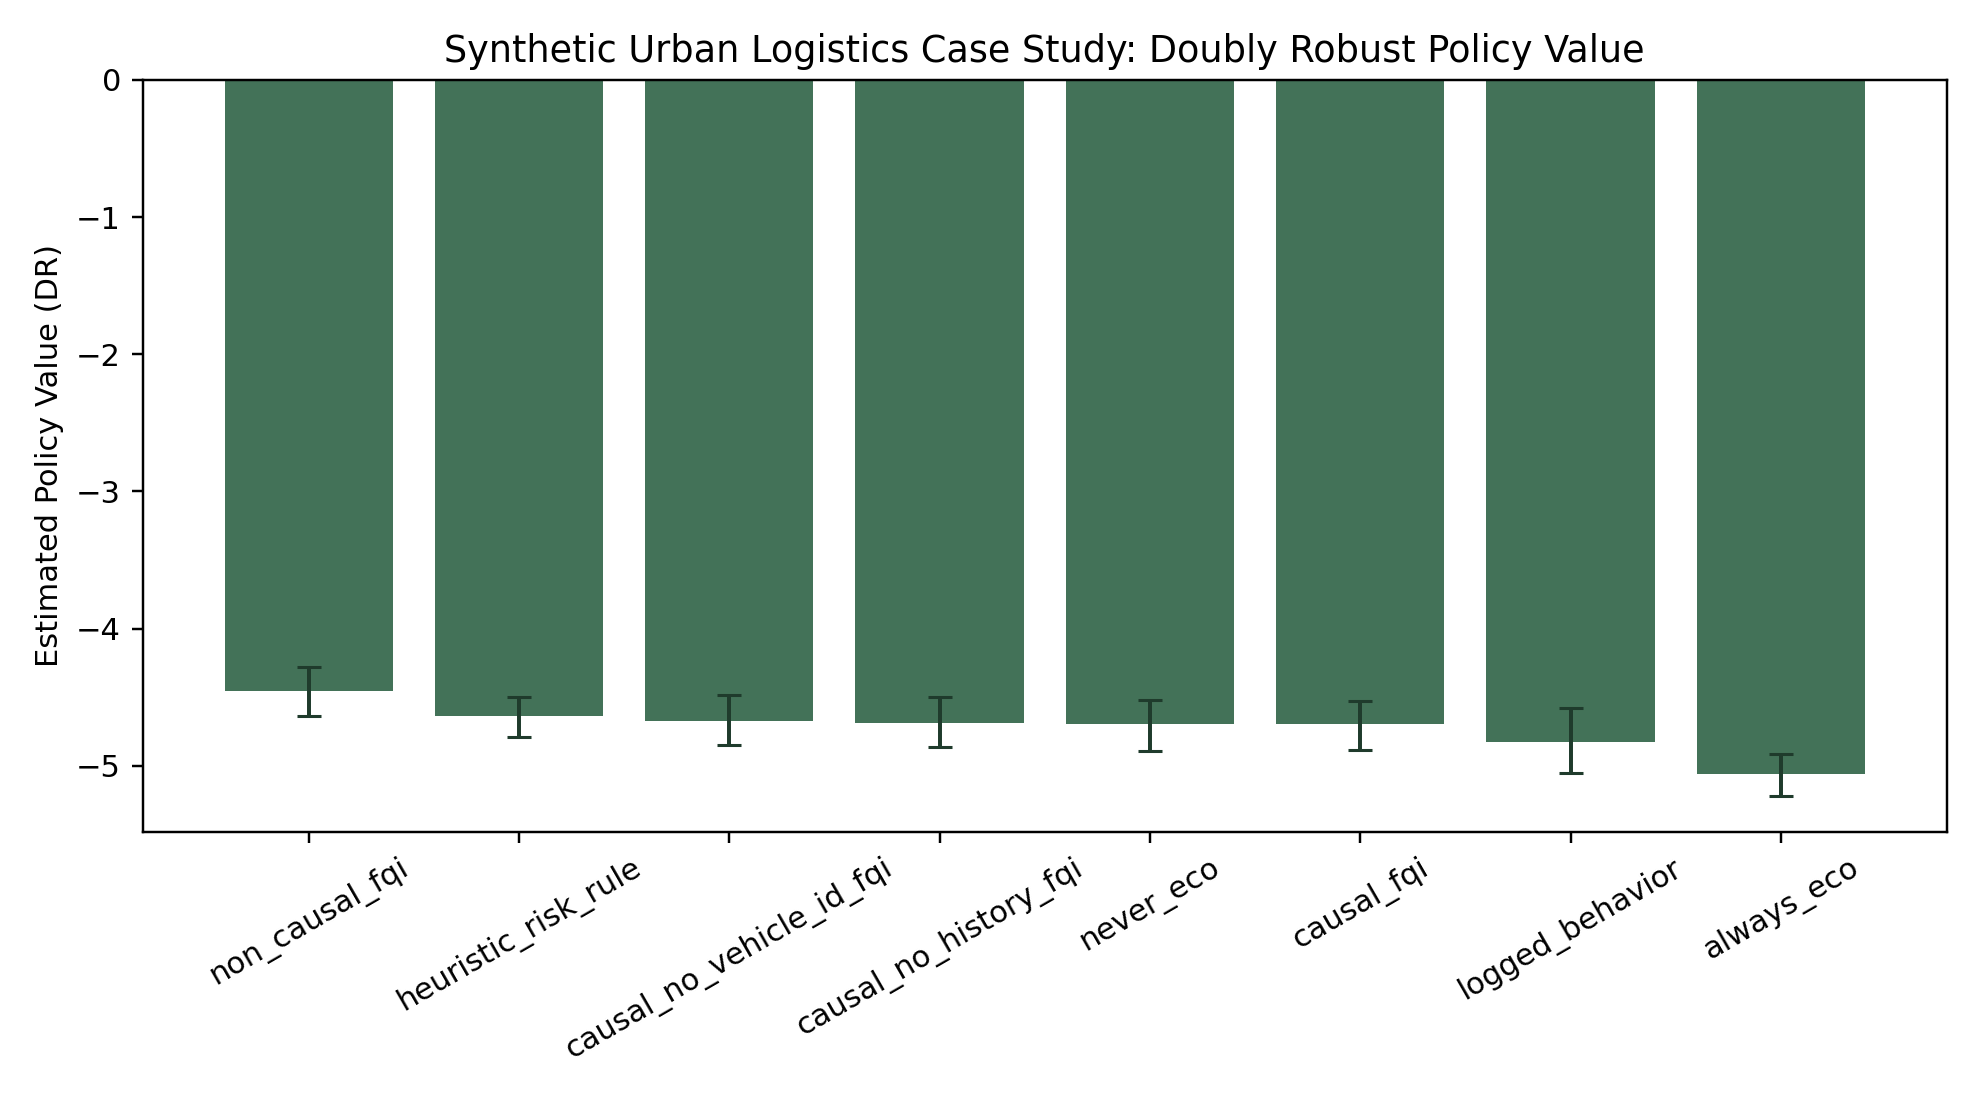
\includegraphics[width=\columnwidth]{policy_values.png}}
\caption{Overall policy-value estimates with bootstrap intervals. Values to the right are better; the dashed line marks held-out logged-action replay.}
\label{fig:policy_values}
\end{figure}

Support thresholds $\tau_\mu = 0.05$ and $\tau_Q = 0.50$ were selected on validation using DR value $-0.5\cdot$override rate $-0.25\cdot$low-support rate. The common-support diagnostic shows minimum propensity $0.023$ with only $0.03\%$ of test rows (4 of 14{,}260) below $\tau_\mu$. Thus, the benchmark supports a proxy-audit reversal over non-causal FQI, not a claim that full confounder-aware FQI is best overall.

A repository-level dominance audit is only a claim-boundary check. It reports 8 counterexamples across 11 audited estimator, reward, and segment surfaces; \texttt{causal\_fqi} is top only on discounted trajectory-return FQE. A controlled DGP is the positive control, where \texttt{causal\_fqi} ranks first by true interventional rollout value. These diagnostics reject strict universal dominance and record a bounded theorem template under conditional exchangeability, overlap, consistent fitted-Q estimation, objective alignment, action relevance, and a positive value gap. This is not a universal theorem: the action-irrelevant MDP counterexample ties all policies, and the theorem-assumption audit leaves main benchmark assumptions unverified.

\subsection{What the Confounder-Aware Framing Contributes}
The confounder-aware framing contributes auditable state-design discipline. It separates deployable pre-decision context from post-action variables, latent simulator columns, \texttt{distance\_km}, and the decision-time-ambiguous \texttt{risk\_score}; \texttt{compatibility\_violation} is retained only in the non-causal comparator. This design produces a proxy-audited FQI comparison reversal, keeps interpretable Q-function drivers, and supports conservative recommendation gating without claiming universal empirical dominance.

\subsection{Ablations and Robustness}
The confounder-aware ablations are stable: removing history changes DR by $+0.007$, removing vehicle identity by $+0.024$, and the 5-feature minimal baseline drops to $-4.810$, a $+0.116$ gap below confounder-aware FQI. A no-fallback greedy sensitivity reaches $-4.675$, while a non-deployable latent-state oracle reaches $-4.550$; these separate support-gate and unobserved-confounding boundaries from the deployable result.

Segment robustness is summarized in Fig.~\ref{fig:robustness}. Non-causal FQI remains above confounder-aware FQI in \emph{high traffic}, \emph{tight window}, and \emph{late day}, while confounder-aware FQI is above it in \emph{rain or event}. Confounder-aware FQI remains above logged replay except in \emph{late day}, where mild shifts in \texttt{traffic\_index} (+0.014) and \texttt{dispatch\_delay\_min} (+0.18 min) increase fallback pressure.

\begin{figure}[t]
\centerline{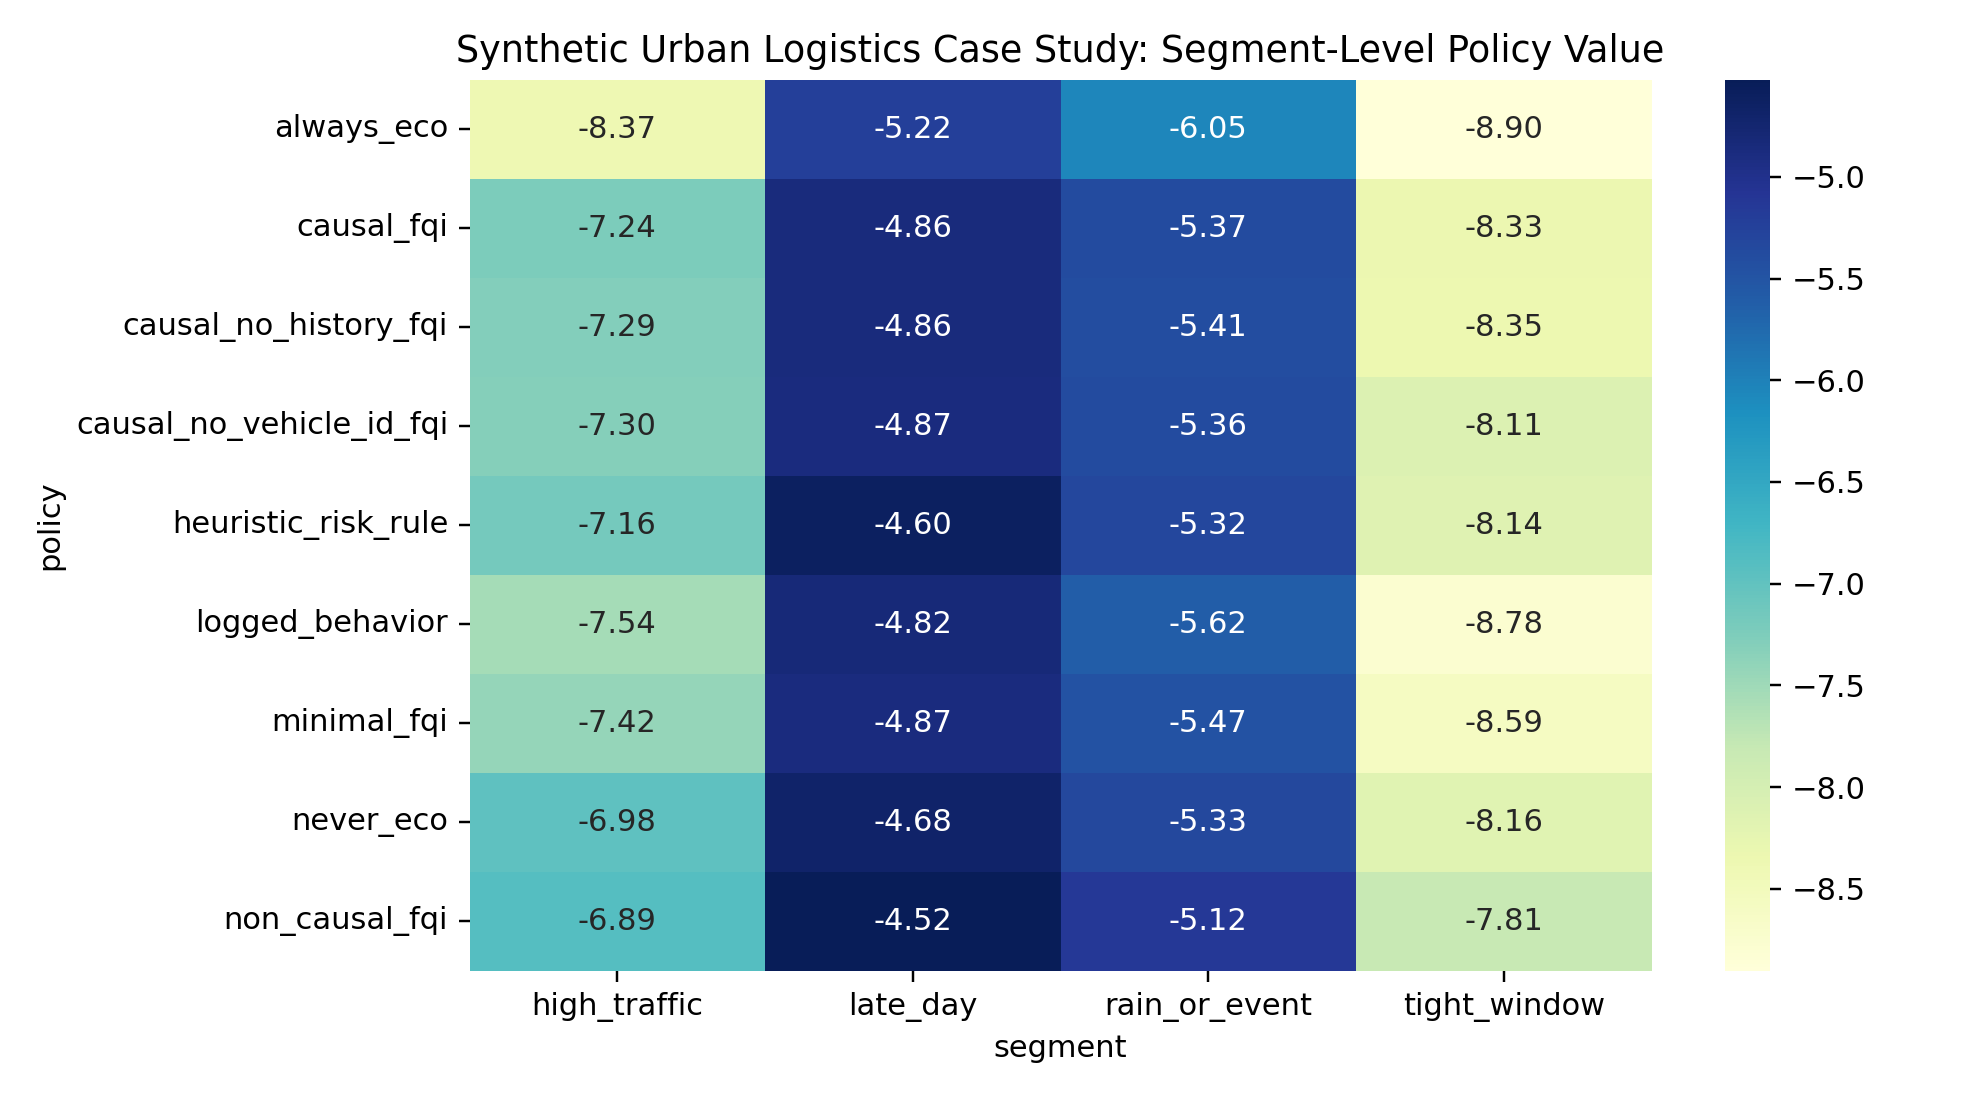
\includegraphics[width=0.95\columnwidth]{robustness_heatmap.png}}
\caption{Per-decision doubly robust reward values by operational segment. Non-causal FQI remains above confounder-aware FQI in three slices, while confounder-aware FQI is above logged-action replay everywhere except \emph{late day}.}
\label{fig:robustness}
\end{figure}

Reward sensitivity reinforces the benchmark's value as an audit tool. The heuristic rule remains strongest under the primary, service-heavy, and sustainability-heavy rewards, while confounder-aware FQI remains above the non-causal FQI comparator and logged-action replay under all three reward specifications. Static and ablated policies change rank, so the benchmark identifies objective-dependent trade-offs rather than one stable global ordering.

\subsection{Practical Interpretation}
The method should be read as a \emph{decision-support layer for eco-mode selection} --- not as a justification for autonomous control. Confounder-aware FQI overrides logged replay on $\sim 26\%$ of test rows and falls back on $\sim 47\%$; the remaining $\sim 28\%$ pass the support/value gate but match the logged action.

For an industrial engineering workflow, the central artifact is the audit trail: deployable state definitions, fitted propensities, override/fallback indicators, segment OPE, regenerated manuscript checks, and a saved-model runtime benchmark, not full training cost. In a field pilot, the same structure would support staged review of recommendation contexts and fallback rates.

\subsection{Threats to Validity}
This study is a synthetic benchmark rather than field validation. The action space is binary, generator equations are unavailable, within-hour ordering uses source-row tie breaks, and three simulator-only latent factors remain unavailable to deployment-time policies. The causal adjustment set is an auditable design choice, not proof that all backdoor paths are blocked. OPE values depend on learned nuisance models, so overlapping intervals warn against strong dominance claims.

\section{Conclusion}
\label{sec:conclusion}
The paper presents eco-mode selection as an auditable synthetic benchmark for confounder-aware decision support. Confounder-aware FQI shows a point-estimate improvement over logged replay, a minimal baseline, and the proxy-audited non-causal FQI comparator while remaining support-constrained. Heuristic and ablated policies can still be stronger, so the contribution is the claim-bounded decision-support workflow and reproducible audit trail rather than a universal dominance claim.

\subsection*{Limitations and Future Work}
The dataset is synthetic, the action space is binary, and there is no live deployment. Future work should test richer actions, partially observable variants, time-of-day-specific policies, real logs, pre-registered support thresholds, shadow-mode recommendations, and prospective service, safety, and emissions outcomes. Separate causal questions, such as the effect of using a one-year-newer vehicle on CO\textsubscript{2}, require a new treatment definition and are not estimated by this eco-mode policy study.

\begin{thebibliography}{99}

\bibitem{demir_green_2014} E. Demir, T. Bektas, and G. Laporte, ``A review of recent research on green road freight transportation,'' \emph{European Journal of Operational Research}, vol. 237, no. 3, pp. 775--793, 2014.

\bibitem{dekker2012or} R. Dekker, J. Bloemhof, and I. Mallidis, ``Operations research for green logistics --- an overview of aspects, issues, contributions and challenges,'' \emph{European Journal of Operational Research}, vol. 219, no. 3, pp. 671--679, 2012.

\bibitem{derrow2021eta} A. Derrow-Pinion \emph{et al.}, ``ETA prediction with graph neural networks in Google Maps,'' in \emph{Proc. 30th ACM Int. Conf. Information \& Knowledge Management (CIKM)}, 2021, pp. 3767--3776.

\bibitem{wang2019simple} H. Wang, X. Tang, Y.-H. Kuo, D. Kifer, and Z. Li, ``A simple baseline for travel time estimation using large-scale trip data,'' \emph{ACM Trans. Intelligent Systems and Technology}, vol. 10, no. 2, Art. no. 19, pp. 19:1--19:22, 2019.

\bibitem{li2018dcrnn} Y. Li, R. Yu, C. Shahabi, and Y. Liu, ``Diffusion convolutional recurrent neural network: Data-driven traffic forecasting,'' in \emph{Proc. Int. Conf. Learning Representations (ICLR)}, 2018.

\bibitem{toth2014vrp} P. Toth and D. Vigo, Eds., \emph{Vehicle Routing: Problems, Methods, and Applications}, 2nd ed. Philadelphia, PA, USA: SIAM, 2014.

\bibitem{pearl2009causality} J. Pearl, \emph{Causality: Models, Reasoning, and Inference}, 2nd ed. Cambridge, U.K.: Cambridge Univ. Press, 2009.

\bibitem{hernan2020causal} M. A. Hern\'an and J. M. Robins, \emph{Causal Inference: What If}. Boca Raton, FL, USA: Chapman \& Hall/CRC, 2020.

\bibitem{lu2018deconfounding} C. Lu, B. Sch\"olkopf, and J. M. Hern\'andez-Lobato, ``Deconfounding reinforcement learning in observational settings,'' 2018, arXiv:1812.10576.

\bibitem{levine2020offline} S. Levine, A. Kumar, G. Tucker, and J. Fu, ``Offline reinforcement learning: Tutorial, review, and perspectives on open problems,'' 2020, arXiv:2005.01643.

\bibitem{ernst2005tree} D. Ernst, P. Geurts, and L. Wehenkel, ``Tree-based batch mode reinforcement learning,'' \emph{Journal of Machine Learning Research}, vol. 6, pp. 503--556, 2005.

\bibitem{fujimoto2019bcq} S. Fujimoto, D. Meger, and D. Precup, ``Off-policy deep reinforcement learning without exploration,'' in \emph{Proc. Int. Conf. Machine Learning (ICML)}, 2019, pp. 2052--2062.

\bibitem{kumar2020cql} A. Kumar, A. Zhou, G. Tucker, and S. Levine, ``Conservative Q-learning for offline reinforcement learning,'' in \emph{Adv. Neural Inf. Process. Syst. (NeurIPS)}, vol. 33, 2020, pp. 1179--1191.

\bibitem{laroche2019spibb} R. Laroche, P. Trichelair, and R. T. des Combes, ``Safe policy improvement with baseline bootstrapping,'' in \emph{Proc. Int. Conf. Machine Learning (ICML)}, 2019, pp. 3652--3661.

\bibitem{prudencio2023survey} R. F. Prudencio, M. R. O. A. Maximo, and E. L. Colombini, ``A survey on offline reinforcement learning: Taxonomy, review, and open problems,'' \emph{IEEE Trans. Neural Netw. Learn. Syst.}, vol. 35, no. 8, pp. 10237--10257, 2024.

\bibitem{bareinboim2016causal} E. Bareinboim and J. Pearl, ``Causal inference and the data-fusion problem,'' \emph{Proc. Natl. Acad. Sci. USA}, vol. 113, no. 27, pp. 7345--7352, 2016.

\bibitem{zhang2019dtr} J. Zhang and E. Bareinboim, ``Near-optimal reinforcement learning in dynamic treatment regimes,'' in \emph{Adv. Neural Inf. Process. Syst. (NeurIPS)}, vol. 32, 2019, pp. 13401--13411.

\bibitem{eglese2014green} R. Eglese and T. Bektas, ``Green vehicle routing,'' in \emph{Vehicle Routing: Problems, Methods, and Applications}, 2nd ed., P. Toth and D. Vigo, Eds. Philadelphia, PA, USA: SIAM, 2014, pp. 437--458.

\bibitem{thomas2015hcpi} P. S. Thomas, G. Theocharous, and M. Ghavamzadeh, ``High confidence policy improvement,'' in \emph{Proc. Int. Conf. Machine Learning (ICML)}, 2015, pp. 2380--2388.

\bibitem{komorowski2018sepsis} M. Komorowski, L. A. Celi, O. Badawi, A. C. Gordon, and A. A. Faisal, ``The Artificial Intelligence Clinician learns optimal treatment strategies for sepsis in intensive care,'' \emph{Nature Medicine}, vol. 24, no. 11, pp. 1716--1720, 2018.

\bibitem{gottesman2019guidelines} O. Gottesman \emph{et al.}, ``Guidelines for reinforcement learning in healthcare,'' \emph{Nature Medicine}, vol. 25, no. 1, pp. 16--18, 2019.

\bibitem{precup2000op} D. Precup, R. S. Sutton, and S. Singh, ``Eligibility traces for off-policy policy evaluation,'' in \emph{Proc. Int. Conf. Machine Learning (ICML)}, 2000, pp. 759--766.

\bibitem{dudik2011dr} M. Dudik, J. Langford, and L. Li, ``Doubly robust policy evaluation and learning,'' in \emph{Proc. Int. Conf. Machine Learning (ICML)}, 2011, pp. 1097--1104.

\bibitem{jiang2016doubly} N. Jiang and L. Li, ``Doubly robust off-policy value evaluation for reinforcement learning,'' in \emph{Proc. Int. Conf. Machine Learning (ICML)}, 2016, pp. 652--661.

\bibitem{thomas2016dataefficient} P. S. Thomas and E. Brunskill, ``Data-efficient off-policy policy evaluation for reinforcement learning,'' in \emph{Proc. Int. Conf. Machine Learning (ICML)}, 2016, pp. 2139--2148.

\bibitem{le2019batch} H. Le, C. Voloshin, and Y. Yue, ``Batch policy learning under constraints,'' in \emph{Proc. Int. Conf. Machine Learning (ICML)}, 2019, pp. 3703--3712.

\bibitem{kallus2020double} N. Kallus and M. Uehara, ``Double reinforcement learning for efficient off-policy evaluation in Markov decision processes,'' \emph{Journal of Machine Learning Research}, vol. 21, no. 167, pp. 1--63, 2020.

\bibitem{prayitno2024framework} K. A. Prayitno and H. Wicaksono, ``Optimizing the sustainability of collaborative logistics in urban area through ontologies and causal artificial intelligence: A conceptual framework,'' \emph{Procedia CIRP}, vol. 130, pp. 1070--1076, 2024.

\bibitem{prayitno2024causalrlreview} K. A. Prayitno and H. Wicaksono, ``Investigating the potential of causal reinforcement learning in collaborative urban logistics: A systematic literature review,'' in \emph{Proc. IEEE Int. Conf. Industrial Engineering and Engineering Management (IEEM)}, 2024, in press, doi: 10.1109/IEEM62345.2024.10857179.

\end{thebibliography}

\end{document}
